% Project synopsis, SPPU B.E. report style: A4, Times 12 pt, one-and-a-half
% spacing, single column, signed title page. Deliberately NOT IEEEtran -- the
% Project Work Book's own formatting annexure prescribes this layout, and the
% signature blocks, Gantt chart and requirements tables do not fit a 3.5 in
% column. The IEEE-format paper is a separate artifact, attached as Annexure A.
%
% IEEE conventions that ARE kept: numbered [n] citations, IEEE reference
% formatting, tables captioned above and figures below, numbered equations.
%
% `times` is not used: tectonic runs XeTeX, which uses the TU encoding, and the
% times package declares no TU shapes -- every glyph silently falls back. newtx
% is the maintained equivalent.
\documentclass[12pt,a4paper]{article}

\usepackage[top=1in,bottom=1in,inner=1.25in,outer=1in]{geometry}
\usepackage{newtxtext,newtxmath}
\usepackage{setspace}
\usepackage{graphicx}
\usepackage{booktabs}
\usepackage{array}
\usepackage{enumitem}
\usepackage{caption}
\usepackage{titlesec}
\usepackage{tikz}
% calc is needed for the ($(node.north west)+(0,0.3)$) coordinate arithmetic that
% places the stage labels; without it tikz fails on the dollar signs.
\usetikzlibrary{arrows.meta, positioning, fit, backgrounds, calc}
\usepackage{microtype}
\usepackage[hidelinks]{hyperref}

\onehalfspacing
% A 6 in measure at 12 pt leaves little room to stretch a justified line; without
% this, several lines run a few points into the margin.
\emergencystretch=1.2em
\captionsetup{font=small,labelfont=bf}
\setlist{topsep=4pt,itemsep=2pt,parsep=0pt}
\titleformat{\section}{\normalfont\large\bfseries}{\thesection}{0.6em}{}
\titleformat{\subsection}{\normalfont\normalsize\bfseries}{\thesubsection}{0.6em}{}

% Every unfilled field is one macro, so `grep PLACEHOLDER Synopsis.tex` finds
% them all and none reaches the printed copy unnoticed.
\newcommand{\PH}[1]{\textbf{[#1 --- PLACEHOLDER]}}

\begin{document}

% ---------------------------------------------------------------- cover page
% The title page must hold everything Annexure i lists AND stay on one page, so
% the spacing here is tight on purpose and the student table is set \small.
\begin{titlepage}
\centering
\singlespacing
\vspace*{0.15in}

{\large A PROJECT SYNOPSIS ON}\\[0.22in]

{\LARGE\bfseries Watermark-Guided Tamper Localization\\[0.08in] and Recovery}\\[0.16in]

{\normalsize A Key-Seeded Self-Embedding Fragile Watermarking Scheme\\
with Joint Localization and Restoration Assessment}\\[0.28in]

{\normalsize SUBMITTED IN PARTIAL FULFILMENT OF THE REQUIREMENTS\\
FOR THE DEGREE OF BACHELOR OF ENGINEERING}\\[0.06in]
{\normalsize (Computer Engineering / Information Technology)}\\[0.28in]

{\large\bfseries SUBMITTED BY}\\[0.12in]

{\small
\begin{tabular}{@{}p{2.7in}p{1.9in}@{}}
\toprule
\textbf{Name of Student} & \textbf{Exam Seat No.} \\
\midrule
\PH{Student 1} & \PH{Seat No.} \\[0.12in]
\PH{Student 2} & \PH{Seat No.} \\[0.12in]
\PH{Student 3} & \PH{Seat No.} \\[0.12in]
\PH{Student 4} & \PH{Seat No.} \\
\bottomrule
\end{tabular}}\\[0.28in]

{\large\bfseries UNDER THE GUIDANCE OF}\\[0.1in]
{\normalsize \PH{Guide Name and Designation}}\\[0.28in]

{\normalsize DEPARTMENT OF COMPUTER ENGINEERING / INFORMATION TECHNOLOGY}\\[0.06in]
{\normalsize AJEENKYA DY PATIL SCHOOL OF ENGINEERING, PUNE}\\[0.06in]
{\normalsize SAVITRIBAI PHULE PUNE UNIVERSITY}\\[0.06in]
{\normalsize ACADEMIC YEAR 2026--27}

\vfill
{\small Project Group ID: \PH{Group ID}\\[0.04in]
Domain: Image Processing / Information Security}
\end{titlepage}

% -------------------------------------------------------- certificate page
\thispagestyle{empty}
\begin{center}
{\large\bfseries AJEENKYA DY PATIL SCHOOL OF ENGINEERING, PUNE}\\[0.06in]
{\large DEPARTMENT OF COMPUTER ENGINEERING / INFORMATION TECHNOLOGY}\\[0.35in]
{\Large\bfseries CERTIFICATE}
\end{center}
\vspace{0.25in}

This is to certify that the project synopsis entitled \textbf{``Watermark-Guided
Tamper Localization and Recovery: A Key-Seeded Self-Embedding Fragile
Watermarking Scheme with Joint Localization and Restoration Assessment''} has
been submitted by \PH{Student names} in partial fulfilment of the requirements
for the award of the degree of Bachelor of Engineering in Computer Engineering /
Information Technology of Savitribai Phule Pune University, during the academic
year 2026--27. The work has been carried out under my supervision and guidance,
and is approved for submission.

\vspace{0.9in}

\noindent
% ragged right: justified placeholder text hyphenates into "PLACE-HOLDER"
\begin{tabular}{@{}>{\raggedright\arraybackslash}p{2.0in}
                  >{\raggedright\arraybackslash}p{1.9in}
                  >{\raggedright\arraybackslash}p{1.7in}@{}}
\hrulefill & \hrulefill & \hrulefill \\
{\small\PH{Guide}} & {\small\PH{Head of Dept.}} & {\small\PH{Principal}} \\
Internal Guide & Dept. of Computer Engg./IT & ADYPSOE, Pune \\
\end{tabular}

\vspace{0.7in}
\noindent
\begin{tabular}{@{}p{2.6in}p{2.6in}@{}}
\hrulefill & \hrulefill \\
Signature, Student 1 & Signature, Student 2 \\[0.5in]
\hrulefill & \hrulefill \\
Signature, Student 3 & Signature, Student 4 \\
\end{tabular}

\vspace{0.5in}
\noindent Place: Pune \hfill Date: \rule{1.4in}{0.4pt}

\newpage

% ------------------------------------------------------------------ abstract
\section*{Abstract}
\addcontentsline{toc}{section}{Abstract}

Editing an image convincingly is now a task of seconds, while the formats in
which images are stored protect nothing about their content. Passive forensic
detectors answer only half of the question a practitioner asks: they may indicate
that a region was altered, but they cannot restore the content that was
destroyed, and their modern learned instances require annotated training corpora,
accelerator hardware at inference time, and produce per-pixel confidence scores
that are not explainable under cross-examination. This project develops the
active alternative. A deterministic, training-free self-embedding fragile
watermarking scheme partitions an image into $8 \times 8$ blocks and hides, in
the two least-significant bit-planes of every block, a 32-bit keyed
authentication tag computed over that block's six most-significant bit-planes,
together with a 96-bit compressed recovery descriptor of a spatially distant
partner block selected by a key-seeded single-cycle permutation. Verification
recomputes each tag; a mismatch localizes tampering at block granularity, and
each flagged block is either rebuilt from the descriptor held by its surviving
partner or marked explicitly unrecoverable rather than fabricated. On a 32-image
corpus, embedding distortion is 43.17~dB PSNR at SSIM 0.9824. Across 768
tamper trials spanning four tamper classes and three tamper ratios, block-level
recall is 1.0000 and pixel-level precision 0.9489, and a null condition of
1{,}802{,}240 block verifications yields zero false positives. In-region recovery
quality remains essentially constant as the tamper ratio grows, from 28.96~dB to
28.38~dB, while whole-image quality falls from 33.79~dB to 17.39~dB, which
identifies mapping coverage rather than descriptor fidelity as the dominant
constraint on recovery. Every verification decision reduces to a single
recomputed keyed hash comparison that any third party holding the key can
independently repeat and check bit for bit.

\vspace{0.15in}
\noindent\textbf{Keywords:} fragile watermarking; self-embedding; tamper
localization; image authentication; content recovery; block mapping; keyed
hashing; image forensics.

\newpage
\tableofcontents
\newpage

% ------------------------------------------------------------------ sections
\section{Introduction}

The evidentiary value of a digital image rests on an assumption that is
increasingly unsafe: that the pixels presented are the pixels captured.
Region-level manipulation --- pasting an object from one photograph into another,
erasing an object with an inpainting tool, or replacing a cropped region with
plausible texture --- is available in free software and, with diffusion-based
generative editors, requires neither skill nor time. The consequences are
concrete rather than hypothetical: a radiological study with a lesion removed, a
vehicle-damage photograph submitted with an insurance claim, a surveillance frame
entered into a legal record, or a remote-sensing tile used in an environmental
dispute all derive their utility from an integrity that the image format itself
does not protect.

Two broad families of countermeasures exist. \emph{Passive} (blind) forensics
analyses the received image alone, searching for statistical inconsistencies in
noise residuals, compression history, colour filter array traces or resampling
artefacts; its modern instances are learned \cite{zhou2018learning,wu2019mantranet}.
\emph{Active} approaches insert authentication information into the image before
distribution, so that verification becomes a decision about self-consistency
rather than an inference about provenance; fragile watermarking belongs to this
second family \cite{wong2001secret,rey2002survey}.

Even a perfect detector answers only half of the practitioner's question. Knowing
precisely \emph{which} pixels of a radiograph were altered does not restore the
diagnostic content that was overwritten, and in the passive paradigm restoration
is necessarily generative: an inpainting network produces content that is
plausible but bears no evidentiary relationship to the original, which is worse
than no restoration at all when the artefact is evidence. What is required is a
mechanism by which the \emph{original} content --- even a coarse approximation of
it --- survives the attack and can be reinstated. Self-embedding watermarking, in
the line of work following Fridrich and Goljan \cite{fridrich1999selfembedding},
provides exactly this: a compressed representation of each region is hidden
elsewhere \emph{within the same image}, so that a spatially localized attack
destroys a region but not its backup.

This synopsis describes a complete, reproducible localization-and-recovery
pipeline built on that principle which evaluates the two capabilities
\emph{together}. Section~2 gives the motivation; Section~3 surveys the literature
and the market; Sections~4--6 define the problem, objectives and scope;
Section~7 presents the methodology and Section~8 the mathematical model;
Sections~9--10 list modules and requirements; Section~11 reports the outcomes
measured to date; and Sections~12--14 give the plan of work, target publication
venues and conclusion.

\section{Motivation and Relevance of the Work}

Three observations motivate this work.

First, \textbf{detection without restoration is insufficient} in exactly those
domains where image integrity matters most. A verifier who learns that a region of
a medical scan was altered still cannot say what was there, and a generative
reconstruction is not an answer because its content is invented.

Second, \textbf{the deployment economics of learned detectors are frequently
understated}: annotated corpora whose bias bounds what the model can see,
accelerator hardware at inference time that excludes embedded devices and hospital
gateways, and outputs that are not explainable under cross-examination. A
per-pixel confidence of $0.78$ is not an argument. By contrast, every positive
detection here is the statement ``the 32-bit keyed tag stored in block $i$ does
not equal the tag recomputed from block $i$'s current content'' --- verifiable,
repeatable and auditable, with no training set, no GPU and no run-to-run variance.

Third, \textbf{the literature tends to report localization and recovery
separately}. Quoting a healthy in-region reconstruction figure without disclosing
what fraction of the flagged region was recoverable at all can flatter a scheme
substantially, so this project treats the joint report --- localization quality,
recoverability rate and recovery fidelity in one table --- as a requirement.

The application domains follow: forensic evidence archives, media authentication
at ingest, medical imaging integrity in PACS, legal and official document scans,
insurance claim verification, and self-authenticating camera or scanner firmware.
All share the property that makes an active scheme viable --- the acquisition
pipeline is under institutional control, so cooperation at capture time is
realistic.

\section{Literature Survey and Market Survey}

\subsection{Passive forensics and learned detectors}

Passive methods analyse the received image alone. Zhou \emph{et al.}
\cite{zhou2018learning} use a two-stream RGB and noise-residual architecture for
splice localization, and ManTra-Net \cite{wu2019mantranet} uses self-supervised
anomaly features to localize forgeries without training on the specific
manipulation type. Their structural advantage is decisive and must be
acknowledged: they need no cooperation from the acquisition device, which no
active scheme can match. Their costs are the annotated corpora, the GPU at
inference, the unexplainable output, and the fact that any restoration they offer
is hallucinated.

\subsection{Active watermarking: robust, fragile, semi-fragile}

Early watermarking optimised \emph{robustness}: Cox \emph{et al.}
\cite{cox1997secure} embed the mark in perceptually significant transform
coefficients so that ownership survives compression and filtering. Authentication
inverts the requirement --- the mark must be fragile, because its failure is the
signal. Wong and Memon \cite{wong2001secret} developed block-wise fragile schemes
with per-block signatures in the least-significant bits, giving localized, blind
verification. The weakness of pure fragility is that it cannot distinguish a
malicious splice from a benign re-save; Lin and Chang \cite{linchang2000} answered
this with an invariant relation between DCT coefficient pairs that quantization
preserves and manipulation breaks, establishing the semi-fragile pattern. The
present work is deliberately fully fragile, and treats the semi-fragile extension
as future scope.

\subsection{Self-embedding and content recovery}

The step from detection to recovery is due to Fridrich and Goljan
\cite{fridrich1999selfembedding}: embed a compressed version of each block inside
the image itself. Their triad --- block-wise compression, key-dependent mapping to
a distant carrier, LSB embedding --- is the direct ancestor of this design. Lin
\emph{et al.} \cite{lin2005hierarchical} added a hierarchical multi-level block
structure verifying at several granularities, improving localization resolution
and the robustness of the tamper decision.

Security analysis runs alongside. Holliman and Memon
\cite{holliman2000counterfeiting} showed that if a block's watermark depends only
on that block's own content, an adversary can collage authentic blocks into a
counterfeit in which every block verifies. Fridrich \cite{fridrich2002security}
analysed localizing fragile marks in the same spirit. The practical consequence,
adopted here without modification, is that the authentication tag must bind block
content, block index and an image-level identifier under a secret key.

\subsection{The tamper coincidence problem}

A one-to-one backup allocation has a characteristic failure: a block and the
block holding its recovery data may be destroyed by the same attack. Aminuddin
and Ernawan named this the \emph{tamper coincidence problem} and, in AuSR3
\cite{ausr3}, addressed it by mapping each block's recovery data to the most
distant available location; the earlier AuSR1 \cite{ausr1} established the
family's $2\times2$ recovery granularity. \textbf{The distant-mapping principle is
theirs, not ours}, and this synopsis does not claim it. What this project
contributes is the specific construction: a key-seeded permutation built directly
in cycle notation, so that bijectivity and the absence of short cycles hold
unconditionally rather than being checked after the fact, combined with an
enforced minimum-separation repair pass.

\subsection{Reference sharing and fountain-coded allocation}

Zhang \emph{et al.} \cite{zhang2011reference} reframed payload allocation so that
reference information is \emph{shared} across blocks and reconstruction becomes
the solution of a linear system, lifting the tolerable tamper ratio above the
naive one-to-one limit. Korus and Dziech \cite{korus2013efficient} added
content-adaptive self-embedding with a formal rate--distortion analysis. This
matters directly to the present design and is stated plainly in Section~11: a
one-to-one mapping fails all-or-nothing per block, whereas shared allocations
degrade gracefully, which is why Korus and Dziech report far higher whole-image
reconstruction at high damage levels than this scheme achieves.

\subsection{Learned proactive watermarking}

A recent family embeds a learned watermark so that a trained network both
localizes and recovers; EditGuard \cite{editguard} is representative, jointly
optimising an invertible watermarking network for localization and copyright
protection. ``Active watermarking detects but does not recover'' is therefore no
longer an accurate description of the field, and this project does not claim
better accuracy than these systems. The distinction offered is auditability: a
decision here is one recomputed keyed hash, reproducible bit for bit by any third
party holding the key, whereas a learned localizer's decision is a trained
network's output and cannot be recomputed without its weights.

\begin{table}[htbp]
\centering
\caption{Summary of the surveyed literature.}
\label{tab:lit}
\small
\begin{tabular}{@{}p{0.4in}p{1.25in}p{1.9in}p{1.75in}@{}}
\toprule
\textbf{Ref.} & \textbf{Author(s), Year} & \textbf{Technique} & \textbf{Limitation / gap} \\
\midrule
\cite{cox1997secure} & Cox \emph{et al.}, 1997 & Spread-spectrum robust watermark in significant coefficients & Robustness is the inverse of authentication; cannot signal change \\
\cite{fridrich1999selfembedding} & Fridrich \& Goljan, 1999 & Origin of self-embedding; compressed backup at a distant carrier & Recovery approximate; no keyed binding of block index \\
\cite{holliman2000counterfeiting} & Holliman \& Memon, 2000 & Counterfeiting attack on block-wise independent marks & Attack, not scheme; forces index and image-ID binding \\
\cite{linchang2000} & Lin \& Chang, 2000 & Semi-fragile authentication via DCT coefficient-pair invariants & Tolerant to compression, so weaker localization precision \\
\cite{wong2001secret} & Wong \& Memon, 2001 & Block-wise fragile signatures in LSBs; blind, localized & Authenticates only; no content recovery \\
\cite{fridrich2002security} & Fridrich, 2002 & Security analysis of localizing fragile marks & Analysis; no recovery mechanism \\
\cite{lin2005hierarchical} & Lin \emph{et al.}, 2005 & Hierarchical multi-level verification & Higher payload cost per block \\
\cite{zhang2011reference} & Zhang \emph{et al.}, 2011 & Reference sharing; reconstruction as a linear system & Higher decode complexity; needs global solve \\
\cite{korus2013efficient} & Korus \& Dziech, 2013 & Content-adaptive self-embedding, rate--distortion analysis & Substantially more complex allocation \\
\cite{ausr1} & Aminuddin \& Ernawan, 2022 & AuSR1: $2\times2$ recovery, LSB shifting & LSB shifting perturbs bits an MSB-authenticating tag must cover \\
\cite{ausr3} & Aminuddin \& Ernawan, 2023 & AuSR3: distant block mapping against tamper coincidence & Comparable per-class recovery figures not citable without re-implementation \\
\cite{editguard} & Zhang \emph{et al.}, 2024 & Learned proactive watermark; localizes and recovers & Requires training and model weights; decision not independently recomputable \\
\bottomrule
\end{tabular}
\end{table}

\subsection{Current market survey}

Deployed products in this space fall into three groups, none of which offers
localization and recovery together from within the image itself.

\textbf{Provenance metadata.} The C2PA Content Credentials standard, adopted by
several camera and editing-software vendors, attaches a cryptographically signed
manifest recording an asset's origin and edit history. Its strength is
standardization and industry backing. Its weakness for this problem is
structural: the manifest lives \emph{beside} the pixels, so re-encoding, a
screenshot, or a metadata strip removes it entirely, and it can never restore
content --- it attests to history rather than protecting it.

\textbf{Controlled-capture services.} Commercial offerings such as Truepic
authenticate images at the moment of capture through a proprietary pipeline. They
give strong provenance where they are used, but require the vendor's software and
infrastructure, and again do not recover destroyed content.

\textbf{Forensic analysis tools.} Analyst-facing products such as Amped
Authenticate, and free services in the FotoForensics mould, apply passive
heuristics --- error-level analysis, noise and CFA inconsistency, metadata
review --- to images with no prior cooperation. Their advantage is that they work
on arbitrary images. Their limitations are that results require expert
interpretation, carry no ground truth, and again offer no restoration.

\textbf{Whole-file digital signatures}, as standardized for DICOM medical imaging,
detect that a file changed but neither localize the change to a region nor
recover it.

The gap in the market mirrors the gap in the literature: existing products either
attest to provenance externally or analyse pixels after the fact, and none embeds
recoverable content inside the image so that a damaged region can be restored
from what survived.

\subsection{Research gap}

The gap addressed here is deliberately narrow, and stating it narrowly is part of
the contribution. It is \emph{not} the distant-mapping idea, which is credited to
AuSR3 \cite{ausr3}. It is \emph{not} superiority over learned proactive
watermarking \cite{editguard}, which already localizes and recovers and against
which no accuracy claim is made. The gap is threefold. First, \textbf{determinism
and auditability}: a construction in which every positive detection reduces to one
recomputed keyed hash comparison that a third party holding the key can repeat
bit for bit, with no training data, no GPU and no run-to-run variance. Second,
\textbf{an explicit keyed construction} with each field binding stated and
analysed, including what each binding defeats. Third, \textbf{joint evaluation}:
imperceptibility, localization and recovery reported together, with the
recoverability rate and the unrecoverable fraction disclosed rather than
excluded, across four tamper classes and three tamper ratios against exact
ground-truth masks.

\section{Problem Definition}

Given a digital image stored in a lossless container and a secret key held by the
authenticating party, embed authentication and recovery information into the
image itself such that: any subsequent region-level modification is localized to
the block grid without reference to the original image or any external database;
the original content of the modified region is approximately restored from
information that survived within the same image; and any region that cannot be
restored is identified as such rather than reconstructed by inference. The
embedding must be perceptually transparent, the verification decision must be
deterministic and independently recomputable, and the entire pipeline must run on
a commodity CPU without trained parameters.

\section{Objectives}

\begin{enumerate}[label=\textbf{O\arabic*.},leftmargin=*]
\item Design a per-block payload that fits entirely within two least-significant
bit-planes, so that embedding distortion is analytically bounded, and achieve mean
imperceptibility of at least 40~dB PSNR over a standard corpus.
\item Construct a key-seeded block mapping that is provably bijective, free of
fixed points and short cycles, and enforces a minimum spatial separation between
a block and its recovery partner.
\item Localize region-level tampering at block granularity with block-level
recall of 1.0 across four distinct tamper classes and three tamper ratios.
\item Produce zero false positives on unmodified watermarked images, verified over
a null condition of more than $10^{6}$ independent block verifications.
\item Reconstruct flagged regions from partner-held descriptors, report an
explicit recoverability rate, and mark unrecoverable regions rather than
fabricating content.
\item Deliver a reproducible evaluation grid and working software, gated by
automated checks that must pass before any result is published.
\end{enumerate}

\section{Scope of the Project}

\textbf{In scope.} Still images, greyscale and three-channel colour, at 8 bits per
channel, stored in lossless containers (PNG, BMP, TIFF). Block sizes 8 and 4.
Two evaluated recovery descriptor designs. Four tamper classes --- copy-paste
splicing, object removal by inpainting, crop-and-refill, and random block
corruption --- at three tamper ratios. A 32-image evaluation corpus. A local web
application and a demonstration interface over the same pipeline.

\textbf{Out of scope.} Video and audio. Robustness to lossy re-encoding,
resizing, rotation or filtering --- the scheme is fully fragile by design.
Adversaries in possession of the secret key, against whom no active scheme can
defend. Real-time embedding in camera firmware, which is an engineering
integration rather than a research question. Comparison against learned detectors
on their own accuracy terms.

\section{Proposed System and Methodology}

\subsection{Overview}

The system has four decoupled stages: embedding at or near acquisition;
tampering, which is simulated by the evaluation harness; verification and
localization at any later point; and recovery. Verification requires only the
received image, the key and the image identifier --- no original, no reference
database, no network call and no model weights.

\begin{figure}[htbp]
\centering
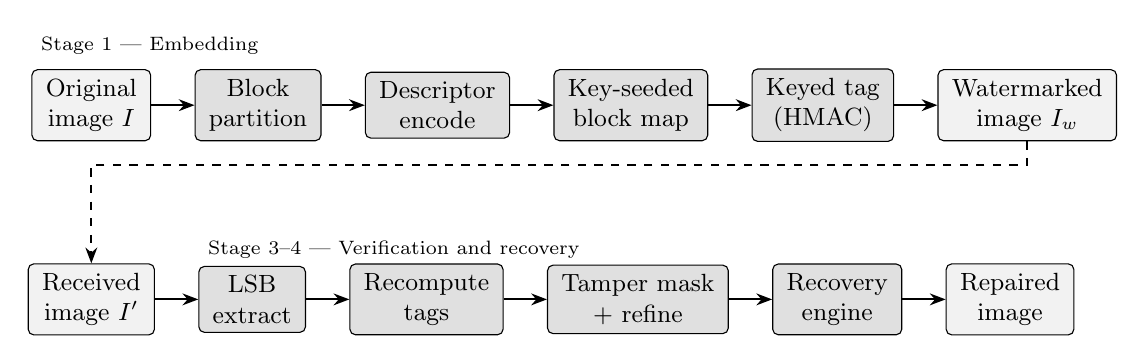
\begin{tikzpicture}[
  node distance=0.42cm and 0.55cm,
  box/.style={draw, rounded corners=2pt, align=center, font=\small,
              minimum height=0.62cm, inner xsep=5pt},
  data/.style={box, fill=black!5},
  proc/.style={box, fill=black!12},
  ar/.style={-{Stealth[length=2mm]}, thick}
]
\node[data] (orig) {Original\\image $I$};
\node[proc, right=of orig] (part) {Block\\partition};
\node[proc, right=of part] (desc) {Descriptor\\encode};
\node[proc, right=of desc] (map) {Key-seeded\\block map};
\node[proc, right=of map] (tag) {Keyed tag\\(HMAC)};
\node[data, right=of tag] (wm) {Watermarked\\image $I_w$};

% 1.55cm, not 1.15: the dashed distribution path runs between the two rows, and
% at the shorter gap it struck through the "Stage 3-4" label.
\node[data, below=1.55cm of orig] (recv) {Received\\image $I'$};
\node[proc, right=of recv] (ext) {LSB\\extract};
\node[proc, right=of ext] (recomp) {Recompute\\tags};
\node[proc, right=of recomp] (loc) {Tamper mask\\+ refine};
\node[proc, right=of loc] (rec) {Recovery\\engine};
\node[data, right=of rec] (out) {Repaired\\image};

\draw[ar] (orig) -- (part);
\draw[ar] (part) -- (desc);
\draw[ar] (desc) -- (map);
\draw[ar] (map) -- (tag);
\draw[ar] (tag) -- (wm);
\draw[ar] (recv) -- (ext);
\draw[ar] (ext) -- (recomp);
\draw[ar] (recomp) -- (loc);
\draw[ar] (loc) -- (rec);
\draw[ar] (rec) -- (out);
\draw[ar, dashed] (wm.south) -- ++(0,-0.30) -| (recv.north);
\node[font=\scriptsize, anchor=west] at ($(orig.north west)+(0,0.30)$) {Stage 1 --- Embedding};
% anchored at the SECOND node: the dashed path drops vertically into recv.north,
% which is exactly where a label anchored at recv would sit, and the line struck
% through the text.
\node[font=\scriptsize, anchor=west] at ($(ext.north west)+(0,0.20)$) {Stage 3--4 --- Verification and recovery};
\end{tikzpicture}
\caption{System architecture. The key $K_s$ and image identifier seed both the
block map and the tag; the dashed path carries the distributed image, which may be
tampered before it reaches verification.}
\label{fig:arch}
\end{figure}

\subsection{Embedding}

The image is partitioned into non-overlapping $B \times B$ blocks in raster order,
with $B = 8$ by default, giving $K = (M/B)(N/B)$ blocks. Dimensions that are not a
multiple of $B$ are cropped rather than padded, so that no synthetic content is
ever authenticated. The two least-significant bit-planes of each block provide
$2B^2 = 128$ bits of capacity, allocated as a 32-bit authentication tag and a
96-bit recovery descriptor.

All hashed and compressed content is computed from the block's six
most-significant bit-planes, obtained by the projection $\mathrm{msb}(a) = a
\wedge \mathtt{0xFC}$. This is the property that makes the scheme single-pass:
because embedding writes only to the two LSBs, it cannot alter what was signed,
so no iterative embed-and-verify loop is required.

The recovery descriptor compresses a block to 96 bits. The primary variant applies
a level-shifted orthonormal two-dimensional DCT and retains the first twelve
zig-zag coefficients, each quantized to a signed 8-bit value using per-band step
sizes taken from the JPEG quality-50 luminance table, giving $12 \times 8 = 96$
bits exactly. A second, low-complexity variant stores a $4 \times 4$ array of
$2 \times 2$ block means at 6 bits each, requiring no transform.

Descriptors are then permuted: block $i$'s descriptor is stored in a distant
partner block, and the tag written into block $i$ binds the descriptor that block
$i$ physically carries. The order matters --- the descriptor is placed first, and
the tag that authenticates it is computed second.

\subsection{Verification, localization and recovery}

Verification extracts the 128 stored bits from each block, splits them into the
stored tag and the stored descriptor, recomputes the tag over the block's current
most-significant content \emph{and the descriptor bits actually present}, and
flags a mismatch. Per-channel decisions are combined by logical OR, so a tamper
touching any single channel flags the block. A neighbourhood refinement pass then
fills isolated negatives, using a threshold scaled by the number of valid
neighbours so that blocks at the image border are not penalised.

Recovery evaluates three sets on a frozen copy of the mask, before any pixel is
written: the flagged set $\mathcal{T}$, the subset $\mathcal{R}$ whose partner is
intact and which can therefore be rebuilt, and the subset $\mathcal{U}$ whose
partner is also flagged. Blocks in $\mathcal{R}$ are decoded from the surviving
descriptor. Blocks in $\mathcal{U}$ are marked with a flat value --- never
inpainted, never silently left in place --- so that a viewer can always tell
reconstructed content from content that could not be recovered.

\section{Relevant Mathematics}

Let $I \in \{0,\dots,255\}^{M \times N}$ be the host image, $K_s$ a secret key,
and $\mathrm{ID}$ an image identifier. Write $b_i$ for the $i$-th block,
$i = 0,\dots,K-1$, and $c(i)$ for its centre coordinate.

\textbf{Bit budget.} For block size $B$,
\begin{equation}
\mathrm{cap}(B) = 2B^2, \quad
t(B) = \min(32,\ \mathrm{cap}(B)/2), \quad
d(B) = \mathrm{cap}(B) - t(B),
\end{equation}
so $B=8$ gives $(128, 32, 96)$ bits of capacity, tag and descriptor respectively.

\textbf{Most-significant projection.}
\begin{equation}
\mathrm{MSB}(a) = a \wedge \mathtt{0xFC},
\end{equation}
which zeroes the two least-significant bits and is idempotent.

\textbf{Block map.} The mapping $m$ is a permutation of $\{0,\dots,K-1\}$
satisfying
\begin{equation}
\text{(R1) } m \text{ bijective}, \quad
\text{(R2) } \lVert c(i) - c(m(i)) \rVert_2 \ge d_{\min}, \quad
\text{(R3) } m \text{ is a single } K\text{-cycle},
\end{equation}
with $d_{\min} = \tfrac{1}{4}\min(M,N)$. R3 is obtained by construction rather
than by rejection sampling: a cryptographically seeded Fisher--Yates shuffle
produces a cycle order, and $m$ is read off it directly, which makes fixed points
and mutual pairs impossible.

\textbf{Descriptor.} With $C_i$ the DCT of the level-shifted projected block and
$\sigma(\ell)$ the zig-zag index,
\begin{equation}
\hat{q}_{i,\ell} = \mathrm{clip}\!\left(\mathrm{round}\!\left(
\frac{C_i(\sigma(\ell))}{\Delta_\ell}\right), -128, 127\right),\;
\ell = 1,\dots,12 .
\end{equation}
No retained coefficient can clip: by Cauchy--Schwarz $|C| \le 1024$ at $B=8$, and
every step size is large enough that the quantized magnitude stays inside the
signed 8-bit range.

\textbf{Authentication tag.}
\begin{equation}
a_i = \mathrm{Trunc}_{32}\Big(\mathrm{HMAC}_{K_s}\big(
\mathrm{ID} \,\Vert\, i \,\Vert\, \mathrm{MSB}(b_i) \,\Vert\, r_{m^{-1}(i)}\big)\Big),
\end{equation}
using SHA-256 \cite{fips180-4}. Each bound field defeats a specific attack:
$\mathrm{MSB}(b_i)$ makes the tag independent of the bits embedding will write;
$i$ and $\mathrm{ID}$ defeat the collage attack of
\cite{holliman2000counterfeiting}; and $r_{m^{-1}(i)}$, the descriptor this block
carries for another, prevents an attacker from replacing recovery data without
detection.

\textbf{Recoverability rate.} With $\mathcal{T}$ the flagged set and
$\mathcal{U} = \{ i \in \mathcal{T} : m(i) \in \mathcal{T} \}$,
\begin{equation}
\rho = 1 - \frac{|\mathcal{U}|}{|\mathcal{T}|} .
\end{equation}

\textbf{Complexity.} Embedding and verification each require one keyed hash and
one $B \times B$ transform per block, plus $O(K)$ for the mapping, giving
$O(MN)$ time overall with no iteration, no optimization and no training. The
problem is therefore of class P; no NP-hard sub-problem arises anywhere in the
pipeline.

\section{List of Modules}

\begin{table}[htbp]
\centering
\caption{Functional modules and their responsibilities.}
\label{tab:modules}
\small
\begin{tabular}{@{}p{1.35in}p{4.0in}@{}}
\toprule
\textbf{Module} & \textbf{Responsibility} \\
\midrule
Payload foundation & Key derivation and domain-separated subkeys, bit budget, block geometry, MSB projection, keyed tag computation, descriptor encoding and decoding, LSB packing. Imported by every other module. \\
Block mapper & Builds the key-seeded single-cycle permutation, enforces the minimum-separation constraint, and verifies R1--R3 before returning. \\
Embedder & Stage 1. Computes descriptors, permutes them, computes the binding tags, writes both into the two LSB planes; asserts that the MSB planes are unchanged. \\
Detector and localizer & Stage 3. Extracts stored payload, recomputes tags, produces the block-level tamper mask, applies neighbourhood refinement, expands to a pixel mask, and exposes a per-block audit record. \\
Recovery engine & Stage 4. Partitions the flagged set into recoverable and unrecoverable, rebuilds the former from partner descriptors, marks the latter, and reports $\rho$. \\
Tamper harness & Generates the four tamper classes with exact ground-truth masks and the achieved tamper ratio. \\
Metrics and evaluation & PSNR, SSIM, confusion counts, localization scores, in-region recovery metrics, and the CSV result grid. \\
Automated gate & Validates the result grid against expected bands and refuses to emit tables or figures if any check fails. \\
Applications & A local web application and a demonstration interface over the same pipeline, with no duplicated numerics. \\
\bottomrule
\end{tabular}
\end{table}

\section{Software and Hardware Requirements}

\begin{table}[htbp]
\centering
\caption{Requirements.}
\label{tab:req}
\small
\begin{tabular}{@{}p{1.35in}p{4.0in}@{}}
\toprule
\textbf{Category} & \textbf{Requirement} \\
\midrule
Language & Python 3.10 or newer. Cryptographic primitives from the standard library (\texttt{hashlib}, \texttt{hmac}, \texttt{struct}); no third-party cryptography. \\
Core libraries & NumPy 2.1.2, OpenCV (headless) 5.0.0.93, scikit-image 0.26.0, Pillow 10.4.0 --- all pinned exactly for reproducibility. \\
Interface libraries & Flask for the local web application; Streamlit 1.61.1 for the demonstration interface; Matplotlib 3.11.1 for figures. \\
Storage & SQLite for the local protected-image library. \\
Document build & \texttt{tectonic} and \texttt{pandoc} (optional; required only to rebuild the paper and this synopsis). \\
Machine learning & \textbf{None.} No framework, no trained parameters, no model artefact to version. \\
Processor & Any commodity x86-64 or ARM CPU. Execution is single-threaded. \\
Accelerator & \textbf{No GPU required at any stage} --- for embedding, verification or recovery. \\
Performance & A $512 \times 512$ image is processed end-to-end in tens of milliseconds on a commodity CPU. \\
Operating system & Platform independent (developed and tested on Windows; no OS-specific dependency). \\
\bottomrule
\end{tabular}
\end{table}

\section{Expected Outcomes and Results Measured to Date}

The evaluation grid comprises \textbf{1{,}184 rows}: 768 main-grid tamper trials
(32 images $\times$ 4 tamper classes $\times$ 3 tamper ratios $\times$ 2
descriptor variants), 320 null-condition rows (32 images $\times$ 2 variants
$\times$ 5 keys), and 96 block-size ablation rows. The corpus is 32 colour
images --- 8 from USC-SIPI \cite{uscsipi} at $512\times512$ and 24 from the Kodak
set --- with every file pinned by SHA-256 so the corpus reproduces byte for byte.
An automated gate reports 23 of 23 checks passing before any figure below is
quoted.

\begin{table}[htbp]
\centering
\caption{Imperceptibility of watermarked images (32-image corpus mean).}
\label{tab:imp}
\small
\begin{tabular}{@{}lcc@{}}
\toprule
\textbf{Descriptor variant} & \textbf{PSNR (dB)} & \textbf{SSIM} \\
\midrule
Variant A (DCT, 12 coefficients) & 43.17 & 0.9824 \\
Variant B (mean-pooled) & 44.23 & 0.9844 \\
\bottomrule
\end{tabular}
\end{table}

\begin{table}[htbp]
\centering
\caption{Localization and recovery against tamper ratio $\alpha$ (Variant A,
averaged over the four tamper classes).}
\label{tab:loc}
\small
\begin{tabular}{@{}lccc@{}}
\toprule
\textbf{Quantity} & $\alpha = 10\%$ & $\alpha = 25\%$ & $\alpha = 50\%$ \\
\midrule
Block-level recall & 1.0000 & 1.0000 & 1.0000 \\
Pixel-level precision (grid mean) & \multicolumn{3}{c}{0.9489} \\
Recoverability rate $\rho$ & 0.9590 & 0.8036 & 0.5335 \\
In-region recovery PSNR (dB) & 28.96 & 28.44 & 28.38 \\
Whole-image PSNR, unmarked (dB) & 33.79 & 23.87 & 17.39 \\
\bottomrule
\end{tabular}
\end{table}

Three results deserve comment.

\textbf{Localization.} Block-level recall is exactly 1.0000 across all 768
main-grid trials. Block-level \emph{precision} is deliberately not headlined:
under the ground-truth rule used here --- a block is tampered if the tamper region
covers any of its pixels --- a block-level false positive is structurally
impossible, so that metric would read 1.000 regardless of detector quality. The
informative figure is pixel-level precision, 0.9489, whose shortfall from 1.0 is
entirely the block-quantization penalty: a flagged $8\times8$ block is reported
whole even when only part of it was altered.

\textbf{The null condition.} Zero false-positive blocks were observed across
1{,}802{,}240 independent block verifications, giving a rule-of-three 95\% upper
bound of $1.66\times10^{-6}$ on the per-block false-positive rate. This is
reported as a determinism and implementation-consistency check across images,
variants and keys --- not as a statistical bound on the $2^{-32}$ cryptographic
false-accept probability, which this experiment does not measure at all.

\textbf{Coverage dominates recovery quality.} In-region recovery PSNR is
essentially flat as the tamper ratio grows (28.96 to 28.38~dB) while whole-image
PSNR collapses (33.79 to 17.39~dB). The two answer different questions: the first
asks how good a reconstructed block is, which the descriptor determines
independently of how many blocks needed reconstruction; the second asks how good
the picture is, which depends on how much of it had to be reconstructed. This is
direct measured evidence that mapping coverage, not descriptor fidelity, is the
dominant lever --- and it identifies reference sharing as the highest-value
upgrade. We state plainly that a one-to-one mapping falls well short of
reference-sharing and fountain-coded schemes at high tamper ratios
\cite{zhang2011reference,korus2013efficient}.

A block-size ablation quantifies the resolution/payload trade-off directly:
reducing $B$ from 8 to 4 raises pixel-level precision from 0.9397 to 0.9736, at a
cost of 2.9~dB of in-region recovery fidelity (29.66 to 26.80~dB), because the
per-block payload falls from 128 to 32 bits and the authentication tag halves.

\section{Project Plan and Schedule}

\begin{table}[htbp]
\centering
\caption{Plan of work. Phases 1--6 are complete; the remainder is scheduled.}
\label{tab:plan}
\small
% Text block is 6.0 in wide; the columns must add up to less than that or the
% Status column prints into the margin.
\begin{tabular}{@{}c p{1.75in} p{2.3in} p{0.85in}@{}}
\toprule
\textbf{Ph.} & \textbf{Activity} & \textbf{Deliverable} & \textbf{Status} \\
\midrule
1 & Literature survey and problem formulation & Survey, gap statement & Complete \\
2 & Scheme design: bit budget, tag construction, block map & Design specification & Complete \\
3 & Implementation of the core pipeline & Embed / detect / recover modules & Complete \\
4 & Tamper harness and metrics & Four tamper classes, exact masks & Complete \\
5 & Full experimental grid and validation & 1{,}184-row result grid, 23/23 gate & Complete \\
6 & Applications and adversarial testing & Web application; two defects found and fixed & Complete \\
7 & Paper preparation and internal review & IEEE-format paper (Annexure A) & In progress \\
8 & Variant~C consolidation into the reported grid & Updated tables and figures & Planned \\
9 & Reference-sharing extension (Future Scope~1) & Prototype and comparison & Planned \\
10 & Final report, demonstration and submission & Report, presentation, viva & Planned \\
\bottomrule
\end{tabular}
\end{table}

\noindent\textbf{Probable date of completion:} \PH{Date, as per departmental
academic calendar}.

\section{Target Publication Venues}

The work is intended for submission to a peer-reviewed venue in image forensics or
multimedia security. Two candidate venues, both appropriate in scope:

\begin{enumerate}[leftmargin=*]
\item \textbf{IEEE International Workshop on Information Forensics and Security
(WIFS)} --- the natural venue for authentication and forensic watermarking, and
the community that publishes the tamper-localization literature surveyed above.
\item \textbf{IEEE International Conference on Image Processing} (ICIP), which has
a broad image-processing scope and a long-established watermarking and forensics
track; the Fridrich and Goljan self-correcting-images paper that founds this line
of work appeared there.
\end{enumerate}

Two further options, should a national or journal venue be preferred: the
\emph{National Conference on Communications} (NCC), and the \emph{EURASIP Journal
on Information Security}. Submission deadlines vary by edition and are to be
confirmed against the current call for papers before selection.

A complete IEEE-format manuscript has already been prepared and is attached as
Annexure~A, so submission is a matter of venue selection and formatting rather
than of new writing.

\section{Conclusion}

This project delivers a deterministic, training-free self-embedding fragile
watermarking scheme that localizes tampering at block granularity and restores a
low-frequency approximation of the destroyed content from information carried
within the image itself. Measured over a 1{,}184-row experimental grid, it embeds
at 43.17~dB PSNR and SSIM 0.9824, achieves block-level recall of 1.0000 and
pixel-level precision of 0.9489, and returns zero false positives across
1{,}802{,}240 block verifications. Its recovery coverage degrades toward $1-\alpha$
for dispersed attacks --- the structural limit of one-to-one backup allocation ---
and this synopsis states that limitation rather than concealing it; adopting a
reference-sharing allocation is the identified next step. The property that
distinguishes the design is not accuracy but accountability: every verification
decision is a single recomputed keyed hash comparison, reproducible bit for bit by
any third party holding the key, which is precisely what an evidentiary
application requires and what a learned detector cannot offer.

\begin{thebibliography}{99}
\small

\bibitem{fridrich1999selfembedding} J. Fridrich and M. Goljan, ``Protection of digital images using self-embedding,'' in \emph{Proc. Symp. Content Security and Data Hiding in Digital Media}, Newark, NJ, USA, May 1999.

\bibitem{cox1997secure} I. J. Cox, J. Kilian, F. T. Leighton, and T. Shamoon, ``Secure spread spectrum watermarking for multimedia,'' \emph{IEEE Trans. Image Process.}, vol. 6, no. 12, pp. 1673--1687, Dec. 1997.

\bibitem{holliman2000counterfeiting} M. Holliman and N. Memon, ``Counterfeiting attacks on oblivious block-wise independent invisible watermarking schemes,'' \emph{IEEE Trans. Image Process.}, vol. 9, no. 3, pp. 432--441, Mar. 2000.

\bibitem{linchang2000} C.-Y. Lin and S.-F. Chang, ``Semi-fragile watermarking for authenticating JPEG visual content,'' in \emph{Proc. SPIE 3971, Security and Watermarking of Multimedia Contents II}, 2000, pp. 140--151.

\bibitem{wong2001secret} P. W. Wong and N. Memon, ``Secret and public key image watermarking schemes for image authentication and ownership verification,'' \emph{IEEE Trans. Image Process.}, vol. 10, no. 10, pp. 1593--1601, Oct. 2001.

\bibitem{rey2002survey} C. Rey and J.-L. Dugelay, ``A survey of watermarking algorithms for image authentication,'' \emph{EURASIP J. Appl. Signal Process.}, vol. 2002, no. 6, pp. 613--621, 2002.

\bibitem{fridrich2002security} J. Fridrich, ``Security of fragile authentication watermarks with localization,'' in \emph{Proc. SPIE 4675, Security and Watermarking of Multimedia Contents IV}, San Jose, CA, USA, Jan. 2002, pp. 691--700.

\bibitem{lin2005hierarchical} P.-L. Lin, C.-K. Hsieh, and P.-W. Huang, ``A hierarchical digital watermarking method for image tamper detection and recovery,'' \emph{Pattern Recognit.}, vol. 38, no. 12, pp. 2519--2529, Dec. 2005.

\bibitem{zhang2011reference} X. Zhang, S. Wang, Z. Qian, and G. Feng, ``Reference sharing mechanism for watermark self-embedding,'' \emph{IEEE Trans. Image Process.}, vol. 20, no. 2, pp. 485--495, Feb. 2011.

\bibitem{korus2013efficient} P. Korus and A. Dziech, ``Efficient method for content reconstruction with self-embedding,'' \emph{IEEE Trans. Image Process.}, vol. 22, no. 3, pp. 1134--1147, Mar. 2013.

\bibitem{wang2004image} Z. Wang, A. C. Bovik, H. R. Sheikh, and E. P. Simoncelli, ``Image quality assessment: From error visibility to structural similarity,'' \emph{IEEE Trans. Image Process.}, vol. 13, no. 4, pp. 600--612, Apr. 2004.

\bibitem{fips180-4} National Institute of Standards and Technology, ``Secure Hash Standard (SHS),'' FIPS Publication 180-4, Aug. 2015.

\bibitem{zhou2018learning} P. Zhou, X. Han, V. I. Morariu, and L. S. Davis, ``Learning rich features for image manipulation detection,'' in \emph{Proc. IEEE/CVF Conf. Computer Vision and Pattern Recognition (CVPR)}, Salt Lake City, UT, USA, Jun. 2018.

\bibitem{wu2019mantranet} Y. Wu, W. AbdAlmageed, and P. Natarajan, ``ManTra-Net: Manipulation tracing network for detection and localization of image forgeries with anomalous features,'' in \emph{Proc. IEEE/CVF Conf. Computer Vision and Pattern Recognition (CVPR)}, Long Beach, CA, USA, Jun. 2019.

\bibitem{ausr1} A. Aminuddin and F. Ernawan, ``AuSR1: Authentication and self-recovery using a new image inpainting technique with LSB shifting in fragile image watermarking,'' \emph{J. King Saud Univ. -- Comput. Inf. Sci.}, 2022.

\bibitem{ausr3} A. Aminuddin and F. Ernawan, ``AuSR3: A new block mapping technique for image authentication and self-recovery to avoid the tamper coincidence problem,'' \emph{J. King Saud Univ. -- Comput. Inf. Sci.}, vol. 35, no. 9, art. 101755, 2023.

\bibitem{editguard} X. Zhang, R. Li, J. Yu, Y. Xu, W. Li, and J. Zhang, ``EditGuard: Versatile image watermarking for tamper localization and copyright protection,'' in \emph{Proc. IEEE/CVF Conf. Computer Vision and Pattern Recognition (CVPR)}, 2024.

\bibitem{uscsipi} University of Southern California, Signal and Image Processing Institute, ``The USC-SIPI Image Database.'' [Online]. Available: \url{https://sipi.usc.edu/database/}

\end{thebibliography}

\vspace{0.3in}
\noindent\textbf{Annexure A.} Full IEEE-format manuscript, prepared in the
IEEEtran conference format and compiled to
\mbox{\texttt{IEEE\_Paper.pdf}} (15 pages), attached separately.

\end{document}
